% !TEX root = ../thesis-example.tex
%
\chapter{Algorithmes interactifs / software}
\label{ch:algorithms}

\cleanchapterquote{One general effect of the digital revolution is that avant-garde aesthetic strategies became embedded in the commands and interface metaphors of computer software. In short, the avant-garde became materialized in a computer.}{Lev Manovitch}{The language of the new media}


\noindent La citation de Lev Manovitch en exergue de ce chapitre en reflète la question centrale: le code est l'élément définissant le fonctionnement d'un \gls{DMI} et si sa nature virtuelle rend son usage très malléable, la nature des objets virtuels que l'on manipule est en grande partie conditionnée par les représentations que l'on se fait de l'interaction musicale. Cependant, les machines ont aussi leur contraintes et limitations, qui influencent la conception des protocoles et les choix d'implémentation. Après avoir présenté le contexte informatique dans lequel s'inscrivent les développements logiciels d'informatique musicale temps-réel, je détaillerai trois développements en lien avec ces questions : 
\vspace{-1em}
\begin{itemize}[noitemsep]
	\item \textbf{le concept de ``modèle intermédiaire dynamique''}, qui au dela des questions de mise en relation de variables, propose un modèle abstrait pour l'interaction geste/son;
	\item \textbf{le protocole MP}, qui propose une solution alternative au \gls{MIDI} pour répondre aux questions d'agencement et de connexions de modules de traitement;
	\item \textbf{la librairie \textit{sagrada}}, qui propose un système original de synthèse granulaire modulaire dans Max contrôlée de manière synchrone ou asynchrone;
\end{itemize}

%%%%%%%%%%%%%%%%%%%%%%%%%%%%%%%%%%%%%%%%%
\section{Matériaux algorithmiques}

\noindent Dans le cas des \glspl{DMI}, les données sont essentiellement :
\vspace{-1em}
\begin{itemize}[noitemsep]
	\item \textbf{des signaux audio}, enregistrés dans des tables d'ondes ou sous forme de flux;
	\item \textbf{des algorithmes}, définissant les opérations mathématisques à effectuer pour traiter les données audio
	\item \textbf{des objets}, définissant les opérateurs, les réglages et xxx todo;
	\item \textbf{un graphe}, définissant l'agencement des opérateurs.
\end{itemize}

Dans les environnements de programmation audio, les flux de données sont généralement séparées en deux types majeurs\footnote{C'est notamment le cas dans Max, SuperCollider, Ableton Live, Csound ... qui traitent le signal par blocs plutôt qu'échantillon par échantillon, pour des raisons d'optimisation.} : 
\vspace{-1em}
\begin{itemize}[noitemsep]
	\item \textbf{des signaux synchrones}, représentant par exemple des signaux audio, échantillonés à une fréquence précise, et traités généralement par bloc dans un \gls{DSP};
	\item \textbf{des événements asynchrones}, arrivant de manière sporadique, tels que les messages \gls{MIDI}, \gls{OSC} ou d'autres types de messages propres au programme;
\end{itemize}

\noindent Ces deux types de flux sont généralement associé aux notions d'\textit{audio-rate} et de \textit{control-rate}, définissant deux granularité indépendantes dans le traitement du signal.


\textbf{keywords} ergodynamisme, résonance, mapping.\\

En général, découplage conceptuel (et logiciel) entre la partie DSP et la partie "contrôle". Dans la réalité, ce n'est pas si simple et c'est la raison pour laquelle ce qui est habituellement rangé du côté "mapping" et du côté "synthèse" est rassemblé dans un seul et même chapitre.


\todo{Présentation de MP, de sagrada et de leur articulation (et par là même de l'articulation entre contrôle et synthèse)}

L’atomisation jusqu’au sample, plutôt que séparation entre DSP et messages de contrôle
=> faust, gen\textasciitilde{ } et cie : l’export vers des plateformes multiples.

\subsection{La notion de mapping}

\noindent Dans le domaine des lutheries numériques, le terme de ``mapping'' est très couramment utilisé pour décrire la relation entre les données issues des capteurs (en particulier de l'interface gestuelle) et les paramètres de la synthèse sonore. 
Le terme de mapping est issu des mathématiques dans lequel il se traduit en français par le terme ``d'application'', c'est à dire de relation entre deux ensembles pour lequel chaque élément du premier (appelé ensemble de départ) est relié à un unique élément du second. Andy Hunt le définit donc dans \cite{hunt_towards_2000} comme \iquote{la liaison ou la correspondance entre les paramètres de contrôle (dérivés des actions de l'interprète) et les paramètres de synthèse sonore}\footnote{``the liaison or correspondence between control parameters (derived from performer actions) and sound synthesis parameters''}.\\
\indent Ce terme a glissé dans l'usage du design d'instrument numérique en raison de la relative simplicité des relations dans les premiers développements et est resté en usage alors que les relations de correspondance sont aujourd'hui bien plus complexes, comme le notait déjà Joel Chadabe en 2002, dans \cite{chadabe_limitations_2002}: \iquote{Le mapping décrit la façon dont un contrôle est connecté à une variable. Mais à mesure que les instruments deviennent de plus en plus complexes pour inclure de grandes quantités de données, une sensibilité au contexte, ainsi que des capacités de génération sonore et musicale, le concept de mapping devient plus abstrait et ne décrit pas les réalités plus complexes des instruments électroniques\footnote{Mapping describes the way a control is connected to a variable. But as instruments become more complex to include large amounts of data, context sensitivity, and music as well as sound-generating capabilities, the concept of mapping becomes more abstract and does not describe the more complex realities of electronic instruments.}.}\\
\indent D'après Hunt et Wanderley \cite{hunt_mapping_2002}, deux directions dans le design de mapping :
\vspace{-1em}
\begin{itemize}[noitemsep]
	\item \textbf{generative mechanisms}, such as neural networks to perform mapping;
	\item \textbf{explicitly defined mapping strategies}.
\end{itemize}

Exemples de schéma de mapping de Wanderley dans \cite{wanderley_escher-modeling_1998}.

\extra{\cite{hunt_mapping_2002}: \iquote{(...) we define mapping as the act of taking real-time performance data from an input device and using it to control the parameters of a synthesis engine.}}

%-----------------------------------
\subsection{Sons de synthèses ou échantillons ?}

\noindent La question est souvent posée, concernant la synthèse sonore de \glspl{DMI}, s'ils utilisent des sons de synthèse ou des sons enregistrés, oubliant dans le même temps que les sons enregistrés sont, lorsqu'ils sont rejoués, des sons de synthèse.\\
\indent Il serait alors tentant de faire une distinction entre des sons synthétisées à partir de purs modèles mathématiques et des sons synthétisés à partir d'échantillons enregistrés dans des tables d'onde. Pourtant, là encore, cette distinction serait vaine
\indent Cette distinction est plus adéquate lorsqu'on parle de synthèse  d'une analogie avec la différence qu'il existe en image vectorielle, composée de primitives géométrique qui la définisse et une image matricielle, définie directement par la matrice de ses pixels.\\
synthèse extensive ou intesive.

\todo{reformuler ça}

%---------------------------------------
\subsection{Synthèse sonore ou contrôle}

Sound  \cite{di_scipio_sound_2003}

\noindent On a tendance à séparer \todo{réf?}, dans la description et le design des \glspl{DMI}, une partie \gls{DSP}, traitant un \textit{signal synchrone}, souvent associée voire confondue à la synthèse audio, et une partie \textit{contrôle}, souvent associé à des données de type \textit{messages asyncrones} (e.g. typiquement, des messages \gls{MIDI}) venant contrôler le \gls{DSP}.\\
\indent Il existe une différence de nature assez profonde entre ces deux types de données, à la fois du côté de leur implémentation technique\footnote{programmation synchrone vs. asynchrone, priorité d'horloge, etc.} mais également dans leur rôle et leur fonction dans l'interaction musicale. 
Ainsi, le signal se présente souvent comme l'\textit{image d'un signal analogique échantillonné} avec l'idée de continuité qui lui est associée. L'autre un graphe asynchrone, se présentant souvent comme l'image d'un ordre d'éxecution (e.g. note-on). \\
\indent D'un côté on a un signal continu et monophonique (un seul échantillon est traité à la fois), de l'autre un signal sporadique et potentiellement polyphonique (plusieurs messages peuvent être envoyé au même instant logique).\\
\indent Cependant, du point de vue de leur utilisation, les frontières entre ces deux types de données numériques d'une part, et ces deux natures d'objets conceptuel (le signal continu et l'ordre événementiel) ne se recouvrent pas exactement. \\
\indent D'une part, il est courant d'utiliser les messages asynchrones de Max pour convoyer des variables continues (telles que les données d'un contrôle MIDI-CC ou d'un capteur envoyé par \gls{OSC}).\\

\todo{Mettre une explication et une ref vers FTM.}

\indent D'autre part, il est également possible d'utiliser un signal synchrone pour déclencher des événements (musicaux) discrets. C'est par exemple le cas lors qu'on envoie une impulsion dans une synthèse de type \gls{KarplusStrong}, ou quand on utilise directement une impulsion audio pour déclencher une enveloppe ou la lecture d'un échantillon.
Cette technique notamment utilisée dans \cite{bascou_gmu_2005} permet de déclencher des flux de grains à haute fréquence (plus rapidement que le système de message de Max ne le permet), ce qui permet notamment de le passage progressif entre flux rythmique et son continu (ref Stockhausen Kontakte)\\
\indent L'arrivée du multi-canal dans le logiciel Max a également conforté cette notion d'utilisation de signaux audio comme messages de contrôle.


%%%%%%%%%%%%%%%%%%%%%%%%%%%%%%%%%%%%%%%%%
\section{Modèles intermédiaires}
\label{sec:algorithms:MID}
Articles du la notion de DIM (@SMC), article sur le jeu de pitch (@ICMC)

\subsection{Motivations}

\noindent Les algorithmes de synthèse et de transformation peuvent présenter un nombre de paramètres trop élevés pour qu'il soit possible de les contrôler individuellement. Diverses méthodes de réduction du nombre de paramètre à gérer par le musicien sur son interface de jeu ont été proposées, telles que l'utilisation de paramètres intermédiaires abstraits \cite{wanderley_escher-modeling_1998}, la projection de l'espace des paramètres sur un espace perceptif \cite{wessel_timbre_1979}, ou d'exploration par voisinage \cite{tubb_divergent_2014}, de modèles physiques \cite{todo}, de modèles d'apprentissage \cite{lee_real-time_1991} \cite{fiebrink_real-time_2011}.

\indent Par ailleurs, la qualité du geste capté ne rend pas forcément compte de la granularité gestuelle qu'on peut observer, par exemple, dans l'interaction fine qui se produit au contact de la surface des matériaux physiques : la souplesse d'un plectre, la rugosité du filetage d'une corde, ou la souplesse du feutre d'un marteau de piano viennent apporter une qualité particulière au son qui ne se résume pas à la vibration d'une corde théorique idéale. Il existe ainsi, dans les instruments acoustiques, divers ``intermédiaires'' entre le geste et le résonateur qui viennent influencer la qualité de leur interaction.\\
\indent Ces systèmes intermédiaires peuvent parfois être interchangeables (on peut jouer sur une guitare avec les doigts, un plectre, un \textit{bottleneck}, etc.) et contribue à élargir la palette de timbres et de styles de jeu d'un même instrument. En transposant cette idée dans le domaine numérique, on peut envisager les modèles intermédiaires dynamiques comme de tels systèmes interchangeables et visant à modifier la qualité des mouvements captés par une interface sensible.

Les modèles génératifs peuvent amener à une liaison trop incertaine entre le geste et le résultat. Les modèles physiques\footnote{Voir par exemple, dans le cas de la synthèse temps-réel les librairies \gls{STK} développée par le \gls{CCRMA} et PMPD initialement développée par Cyrille Henry.} sont une alternative qui pallie ces deux problèmes en offrant à la fois un modèle intermédiaire entre le geste et le résultat qui réduit le potentiellement grand nombre de paramètres de synthèse à un plus petit nombre de paramètres gestuels.\\
\indent Un problème des modèles physiques est d'une part leur instabilité dans les régimes non-linéaires et d'autre part, que la cohérence de la relation entre le geste et le son souhaitée par le musicien ne s'appuie pas nécessairement sur les règles de la mécanique newtonienne \footnote{On pourrait dire à certain égards que les instruments de musique cherchent à subvertir les lois de la physique, cf. section \ref{sec:gesture:subversion}}. Par exemple, on peut assigner à un modèle géométrique des mouvements, un tempo, une cinétique qui épousent la géométrie de l'objet sans toutefois qu'il y soit question de masse et que l'objet ait une ``cohérence physique''.

\subsection{Caractéristiques souhaitées}

\noindent Les MIDs sont ainsi définis par les caractéristiques suivantes:
\vspace{-1em}
\begin{itemize}[noitemsep]
	\item \textbf{enrichir le geste} capté avec des modulations opérant à des fréquences au-delà des fréquences gestuelles humaines (par ex. rebonds rapides);
	\item \textbf{démultiplier le geste} et pouvoir, à partir d'un seul geste d'entrée, contrôler une multitude d'agents;
	\item une intégration facile dans une architecture logicielle modulaire, qui permette de tester et ajuster ses modèles en direct;
	\item la possibilité de piloter simultanément différents moteurs de synthèse et de rendu avec les mêmes algorithmes, afin d'améliorer la cohérence de l'ensemble;
	\item être bidirectionnel : le modèle intermédiaire doit pouvoir communiquer dans les deux sens avec l'interface, les autres DIM ou le moteur de synthèse (cf. Fig. 1) afin de réguler les interactions (non linéaires) entre les différents étages.
\end{itemize}

Les processus à l'œuvre dans un modèle intermédiaire agissent sur plusieurs aspects de la transduction de mouvement attendue dans un instrument de musique.
\vspace{-1em}
\begin{itemize}[noitemsep]
	\item qualité du mouvement: Pour donner un exemple acoustique, un plectrum pour une corde
offre une qualité de pincement particulière et son attaque est différente de celle des doigts. De plus, la position des cordes sur le corps de l'instrument permet de transformer le mouvement apparemment linéaire de la main en une variation de ce mouvement particulier, à savoir une succession de pincées dont le rythme est lié à l'espacement des cordes. Les dispositifs d'interaction sont souvent dépourvus de rugosité de surface (par exemple, une tablette à stylo n'a pas la rugosité du crin d'un archet). Un DIM devra intégrer cet "aspect de surface" de l'objet virtuel.
	\item mouvements non linéaires : La richesse du son est en partie liée à l'ensemble des phénomènes non linéaires en action dans un instrument de musique et contribue à rendre le son riche et subtil. Ces non-linéarités dues en partie aux matériaux des instruments acoustiques (et électroniques) manquent souvent des valeurs numériques standardisées des paramètres des instruments logiciels. Dans le domaine numérique, les non-linéarités se retrouvent en effet souvent dans les bugs et les abus de codecs, toutes sortes de "pépins" qui sont précisément recherchés par une veine de musique électronique portant désormais ce nom, pour produire des sonorités riches et des paysages sonores imprévus. Le DIM devrait donc réintroduire la saturation, les courbes exponentielles, la distorsion et autres gigue dans les fonctions de transfert des instruments numériques. 
	\item Mouvement augmenté : En agissant sur des modèles complexes, un modèle unidimensionnel
peut être convertie en un mouvement polyphonique multidimensionnel. Par exemple, sur un instrument à cordes, les nombreuses notes d'un accord peuvent être jouées d'une seule touche. Ce renforcement du mouvement peut agir sur les dimensions verticales (poly-phoniques), horizontales (polyrythmiques) ou sur les nombreuses dimensions du timbre. On peut par exemple contrôler un "paramètre cible" qu'un ensemble d'éléments atteindrait par une logique de déplacement qui leur est propre.
\end{itemize}

\subsection{Implémentation}
Première implémentation en 2009.
Re-implémentation avec MP.

\subsection{Evaluation}
Utilisation dans la MM. Utilisation dans FIB\_R pour contrôler image et son.


%%%%%%%%%%%%%%%%%%%%%%%%%%%%%%%%%%%%%%%%%
\section{MP : un protocole de connexion modulaire, polyphonique, expressif}
\label{sec:algorithms:MP}

\subsection{Résumé}

\noindent Nous présentons le système MP, un protocole et un ensemble d'outils facilitant la connexion modulaire de processus polyphoniques. Le but de cette librairie est d'améliorer la modularité en conservant les blocs individuels de traitement polyphonique indépendants du mapping général qui a lieu dans le design de l'interaction d'un instrument de musique numérique. Le protocole MP est fondé sur un paradigme à trois états permettant la modulation expressive de tout paramètre. Une stratégie originale est proposée pour le groupement hiérarchique d'événements en spécifiant quels événements ``invités'' seront autorisés à modifier les paramètres d'une voix de polyphonie affectée à cet événement. Une revue préalable des principaux protocoles qui ont inspiré ces développements permettra d'en expliciter les enjeux. Quelques exemples seront donnés pour expliciter les possibilités offertes par cette stratégie. Les développements présentés ici sont implémentés dans le logiciel Max mais la logique sous-jacente reste applicable dans d'autres systèmes utilisant une logique de communication asynchrone.

\indent Les instruments de musique numérique nous mettent face à une équation bancale. D'un côté quelques flux de données issus de capteurs rendent péniblement compte de la finesse du geste physique, de l'autre la possibilité (et le désir) de produire une musique plus complexe qu'aucun instrument acoustique ne peut le faire. La réponse à cette équation réside dans la question centrale de ce que l'on nomme habituellement le \gls{mapping}, c'est à dire la relation de correspondance entre valeurs issues de capteurs et paramètres de synthèse. Cependant, et malgré sa popularité\footnote{Entre 2001 et 2015, le terme "mapping" a été employé dans plus de 750 articles de la conférence \gls{NIME} alors que "design d'interaction" (interaction design) n'était employé que dans 160 articles.}, le terme de mapping semble assez peu représenter la complexité de ce qui n'est pas une simple mise en relation et nous préférerions parler d'un design d'interaction, c'est à dire d'une programmation des relations entre gestes et sons faisant intervenir modèles dynamiques, scénarios évolutifs, fragments de partitions et réglages d'un nombre extrêmement élevé de variables.\\
\indent Nous avons vu dans la section précédente comment le concept de modèle intermédiaire dynamiques pouvait enrichir le geste capté et améliorer l’ergonomie des instruments de musique numériques. Cependant, un des facteurs critiques rencontré lors de ces développements se situait dans la manière de faire communiquer différents modules polyphoniques\footnote{Par « module polyphonique », on entend ici des processeurs traitant simultanément plusieurs flux de données de contrôle de même nature en parallèle, e.g. le filtrage des points de contact sur une interface multi-touch ou encore la modulation des différentes notes d'un accord.} entre eux. L'objectif de MP est donc de rendre cette communication polyphonique, tout en gardant la traçabilité et l'ordonnancement des événements.

%---------------------------------------------------------------------------
\subsection{Motivations et revue des protocoles existants}

\noindent Les protocoles de contrôles que nous envisageons ici sont asynchrones, fondés sur l’idée que les systèmes musicaux envisagés dans les lutheries actuelles sont des systèmes complexes composés d’éléments hétérogènes et intégrant notamment des interfaces \textit{hardware} elle-mêmes asynchrones. Bien que la synthèse audio soit un processus synchrone, le design global d'un \gls{DMI} est le plus souvent un système \iquote{globalement asynchrone, localement synchrone}, tel que défini par Daniel M. Chapiro \cite{chapiro_globally-asynchronous_1984}.\\
\indent Un certain nombre de protocoles dédiés au contrôle temps-réel de la synthèse numérique ont vu le jour depuis les années 1980. Au delà de proposer des solutions techniques concrètes, ces protocoles sont porteurs d’un modèle implicite représentant les objets en présence dans l’interaction geste/son. Une brève revue montrera comment ceux-ci se sont progressivement ouverts, à mesure que les capacités de calcul se sont accrues et que la notion même d’instrument s’élargissait à de nouveaux champs tels que les installations sonores ou les applications musicales interactives.

\subsubsection{MIDI}

\noindent Le \gls{MIDI} a fêté son trentième anniversaire en restant le protocole le plus répandu pour le contrôle de la synthèse audio. La profusion de nouvelles interfaces et applications l'auront tout juste fait évoluer pour permettre la prise en charge de nouvelles technologies de réseau (rtpMIDI\footnote{ Encapsulation du \gls{MIDI} dans des messages \gls{RTP} permettant une communication sur des réseaux ethernet et WiFi.}) ou de nouvelles interfaces (\gls{MPE}, voire sections suivantes)).
Les limitations du \gls{MIDI} ont pourtant été identifiées peu de temps après son apparition \cite{mcmillen_zipi_1994}\cite{moore_dysfunctions_1988}\cite{selfridge-field_beyond_1997}, notamment :
\vspace{-1em}
\begin{itemize}[noitemsep]
	\item sa précision et son espace de nommage sont limités;
	\item l'identifiant d'une note est assimilé à son (éventuelle) hauteur;
	\item l'état actif d'une note est assimilé à sa vélocité;
	\item la modulation individuelle des notes est fastidieuse;
	\item sa nomenclature fait référence aux instruments acoustiques.
\end{itemize}

\noindent Le \gls{MIDI} élude une partie de la question du mapping en reliant intrinsèquement le geste à la production sonore à travers le concept de note \gls{MIDI}\footnote{ Une note \gls{MIDI} est composée d'une valeur de pitch et d'une valeur de vélocité associées à canal \gls{MIDI}.} qui assimile les deux côtés de l'interaction : la notion de vélocité se rapportant au geste et celle de pitch au son.

\subsubsection{ZIPI}

\noindent En 1994, Zeta Instruments et le \gls{CNMAT} proposèrent \gls{ZIPI}\cite{mcmillen_zipi_1994} pour dépasser les limitations du MIDI. \gls{ZIPI} fait ainsi la distinction entre note, hauteur, canal et vélocité, augmente la précision des données, introduit des messages de modulation par note, la possibilité d'un réseau en étoile (plutôt que le chaînage linéaire \gls{MIDI}) ainsi qu'une méthode d'interrogation des instruments connectés.\\
\indent \gls{ZIPI} propose également une organisation hiérarchique à trois niveaux héritée d'une classification traditionnelle où des \iquote{orchestres} sont des ensembles de \iquote{familles d'instruments}, composées \iquote{d'instruments}, proposants un ensemble de \iquote{notes}. ZIPI introduit enfin deux espaces de nommage distincts pour la description du geste d'une part et de la synthèse audio d'autre part.\\
Malheureusement, le public ciblé —les fabricants et utilisateurs de synthétiseurs hardware— n'était pas prêt pour un tel changement alors que l'avènement du protocole \gls{firewire} cette même année palliait le faible débit de données du \gls{MIDI}\footnote{ Le débit d'un bus \gls{MIDI} était jusqu'alors de 31,25 kbit/s en connection DIN uni-directionnelle; le \gls{firewire} proposait jusqu'à 400Mbit/s tout en étant bi-directionnel.}.

\subsubsection{OSC : Open Sound Control}

\noindent En 1997 au \gls{CNMAT}, un groupe incluant d'anciens concepteurs de ZIPI ré-utilisa la recherche menée pour développer le protocole \gls{OSC} \cite{wright_open_1997}, motivé par le besoin de répondre à l'évolution des technologies de réseau et l'extension des types de données alimenté par l'utilisation grandissante de logiciels comme Max. En proposant une syntaxe intelligible et facile à utiliser, \gls{OSC} a connu un certain succès: il a été adopté par un certain nombre de logiciels et interfaces hardware\footnote{ Comme le Lemur, le Monome ou l'Ethersense.} et utilisé pour définir d'autres protocoles tels que \gls{GDIF}, \gls{TUIO}, ou encore la librairie ``o.''\footnote{ « Oh dot » : package pour Max, développée au \gls{CNMAT}.}.\\
\indent Cependant, sa relative lourdeur en terme de débit comparé au \gls{MIDI} \cite{fraietta_open_2008} et une absence de nomenclature rendant fastidieuse les branchements plug'n play l'ont pour l'instant privé d'une adoption par l'industrie et le grand public.

\subsubsection{TUIO: Tangible User Interface I/O}

\noindent Dans cette brève revue, il faut mentionner \gls{TUIO} \cite{kaltenbrunner_tuio:_2005} (fondé sur \gls{OSC}) comme le premier protocole\todo{vérifier à quel point c'est le premier} à introduire un indice incrémentiel pour identifier de manière unique des événements dynamiques et éphémères tels que les touchés de doigt sur une interface utilisateur tangible (\gls{TUI}).\\
\indent Il se distingue également de la logique des événements \gls{MIDI} —dont l'utilisation de messages distincts pour les note-on et -off peut produire des notes qui restent "bloquées" si un message note-off est perdu— en proposant une solution simple et pratique pour résoudre l'incertitude d'arrivée des messages envoyés sur \gls{UDP} et consistant à envoyer systématiquement la liste des événements actifs.

\subsubsection{\gls{MPE}: MIDI Polyphonic Expression}

\noindent La dernière évolution du \gls{MIDI} a été motivée par la commercialisation récente d'interfaces dites expressives\footnote{ Citons le LinnStrument, Roli Seabord, Haken Audio’s Continuum, Eigenharp Alpha, Madrona Labs’ Soundplane, le KMI K-Board Pro4 ou prochainement Joué.}, c'est à dire permettant la modulation indépendante de chaque note jouée. Bien qu'elles ne soient pas les premières interfaces permettant un tel contrôle, un effort conjoint a été entrepris par plusieurs fabricants pour définir standard nommé \gls{MPE}. Cette évolution n'est cependant qu'une normalisation de l'usage des canaux \gls{MIDI} actuels permettant un tel contrôle dans le cadre existant, et non un nouveau protocole qui dépasserait les limitations intrinsèques au \gls{MIDI}.

\subsubsection{Le signal}

\noindent S'il n'est traditionnellement pas envisagé tant comme un signal de contrôle que comme un support pour le signal audio, le signal peut être considéré comme un signal de contrôle synchrone, en valeur flottante. Le développement de la librairie ``Sagrada'', présentée dans la section \ref{sec:algorithms:sagrada}, en donne un example.\\
\extra{quote David Zicarelli lors de la présentation de mc.* présentant le signal comme outil de contrôle.}


%-----------------------------------------------------------------------------------
\subsection{Description générale}

\noindent Un facteur ayant contribué au succès d'un logiciel comme Max est la possibilité qu'il laisse de pouvoir brancher plus ou moins n'importe quelle variable sur une autre, permettant ainsi une grande souplesse dans l'élaboration de scénarios d'interaction ainsi qu'une approche expérimentale des relations de correspondances.
\indent Cependant, la gestion de processus polyphoniques y reste plus délicate. Si un objet comme \textasciitilde{ } permet effectivement de créer des instances multiples d'un même processus, son adressage reste fastidieux\footnote{La gestion de la polyphonie a été améliorée par la prise en charge de messages au format \gls{MPE}, ainsi que par l'ajout de signaux audio polyphoniques dans la dernière version. Cependant, le format \gls{MPE} reste contraint par les limites pré-citées}. En particulier, la distribution d'un processus polyphonique dans plusieurs modules élémentaires indépendants --~ ce qui permet leur ré-agencement~-- n'est pas intégrée de manière native.
\indent MP (\textit{Modular Polyphony})\footnote{Disponible sur: \url{https://github.com/LAM-IJLRA/ModularPolyphony}} est composé de modules de traitement polyphoniques et d'un protocole de messages permettant leur adressage. Il s'inspire de certaines des idées présentes dans les protocoles pré-cités. En particulier, il reprend un concept général du \gls{MIDI} qui conçoit le contrôle musical temps-réel comme une séquence temporelle de \textit{notes} ayant un début et une fin. Il emprunte aussi à \gls{ZIPI} l'idée d'un découplage entre identifiant, hauteur, vélocité, canal ainsi que la nuance entre l'activation d'une note et sa modulation. Par ailleurs, comme ce framework est destiné à une lutherie expérimentale et exploratoire, MP laisse le typage et l'espace de nommage des paramètres ouverts, sans le restreindre à une nomenclature arbitraire. Néanmoins, il propose une syntaxe plus restrictive qu'\gls{OSC} permettant une gestion cohérente et facilitée de la polyphonie. Enfin, MP permet l'association dynamique d'événements entre eux, de tel sorte qu'il soit possible de contrôler les paramètres par groupes (et sous-groupes).\\
\indent MP se compose de blocs de traitement polyphonique nommés \textit{mp-blocks}, communiquant par des messages asynchrones nommés \textit{mp-messages} et représentant des objets temporels abstraits nommés \textit{mp-events}. Les sections suivantes décrivent ces éléments en détail.


%-----------------------------------------------------------------------------------
\subsection{mp-events}

\noindent Un \textit{MP-event} est un objet temporel abstrait qui peut être traité par des \textit{mp-blocks}. Il est défini par un ensemble de \textit{MP-messages} (figure \ref{fig:algorithms:MP-event-model}). Ces messages sont composés de paramètres de contrôle précédés par un identifiant unique propre au \textit{MP-event}. Le format de message est minimaliste et tous les messages utilisent la même syntaxe : un identifiant unique, un nom de paramètre suivi d'une liste de valeurs. Par exemple :
\vspace{-1em}
\begin{itemize}[noitemsep]
	\item{[42 pitch 112] : le \textit{MP-event} \#42 règle le paramètre de pitch à la valeur 112;}
	\item{[123 scale 0 2 4 5 7 9 11] : le \textit{MP-event} \#123 définit une gamme diatonique.}
\end{itemize}
\todo{formater les messages code en verbatim et ou avec une box}

\noindent Deux noms de paramètre sont réservés pour un usage particulier: \texttt{state} et \texttt{guests}. Ils seront détaillés dans les prochaines sections. Nous verrons également qu'un \textit{MP-event} peut suivre plusieurs chemins de traitement en parallèle et être fusionné avec d'autres \textit{MP-event}. 

%------------------ Figure : MP-event et MP-block ---------------------
%\begin{figure}[!htbp]
%	\captionsetup{format=plain}%
%	\centering
%	\begin{minipage}[t]{0.48\textwidth}
%		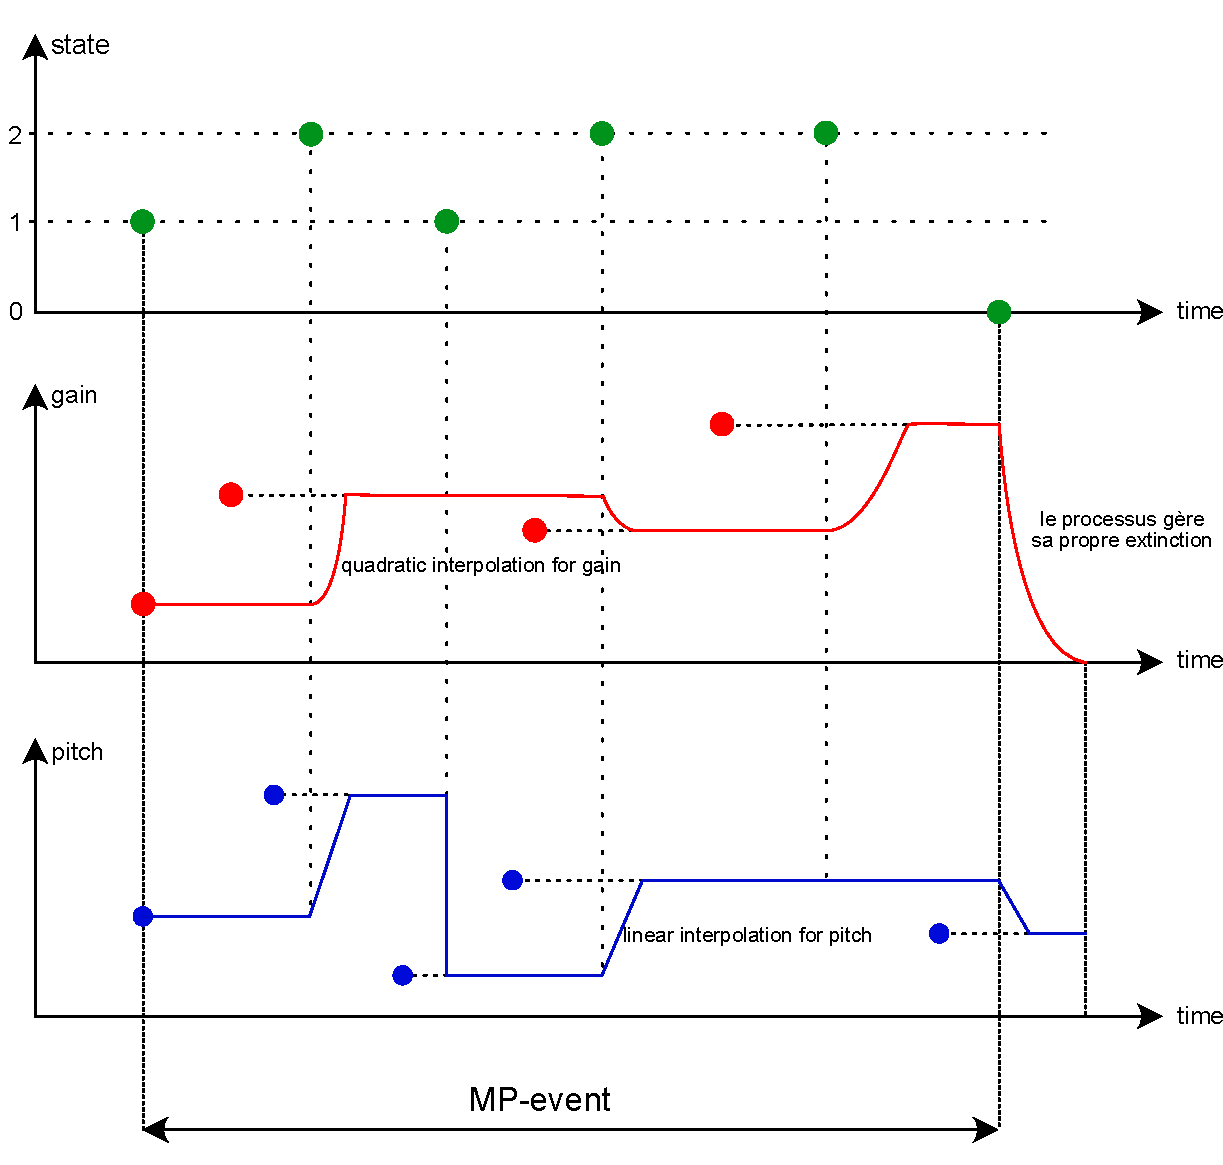
\includegraphics[width=\linewidth]{gfx/04_algorithms/MP-event-model.pdf}
%		\caption[Représentation schématique d'un \textit{MP-event}]{Représentation schématique d'un \%textit{MP-event}. Les cercles pleins représentent les états \textit{on}, les cercles vides les %états \textit{off} et les lignes continues les états \textit{update}.}
%		\label{fig:algorithms:MP-event-model}
%	\end{minipage}
%	\hspace{.02\linewidth}
%	\begin{minipage}[t]{0.48\textwidth}
%	  
\includegraphics[width=\linewidth]{gfx/dummy.pdf}
%		\caption[dummy]{dummy}
%		\label{fig:algorithms:dummy-1}
%	\end{minipage}
%\end{figure}
%------------------ Figure : MP-event et MP-block ---------------------

%------------------ Figure : MP-event ---------------------
\begin{figure}[!htbp]
	\captionsetup{format=plain}
	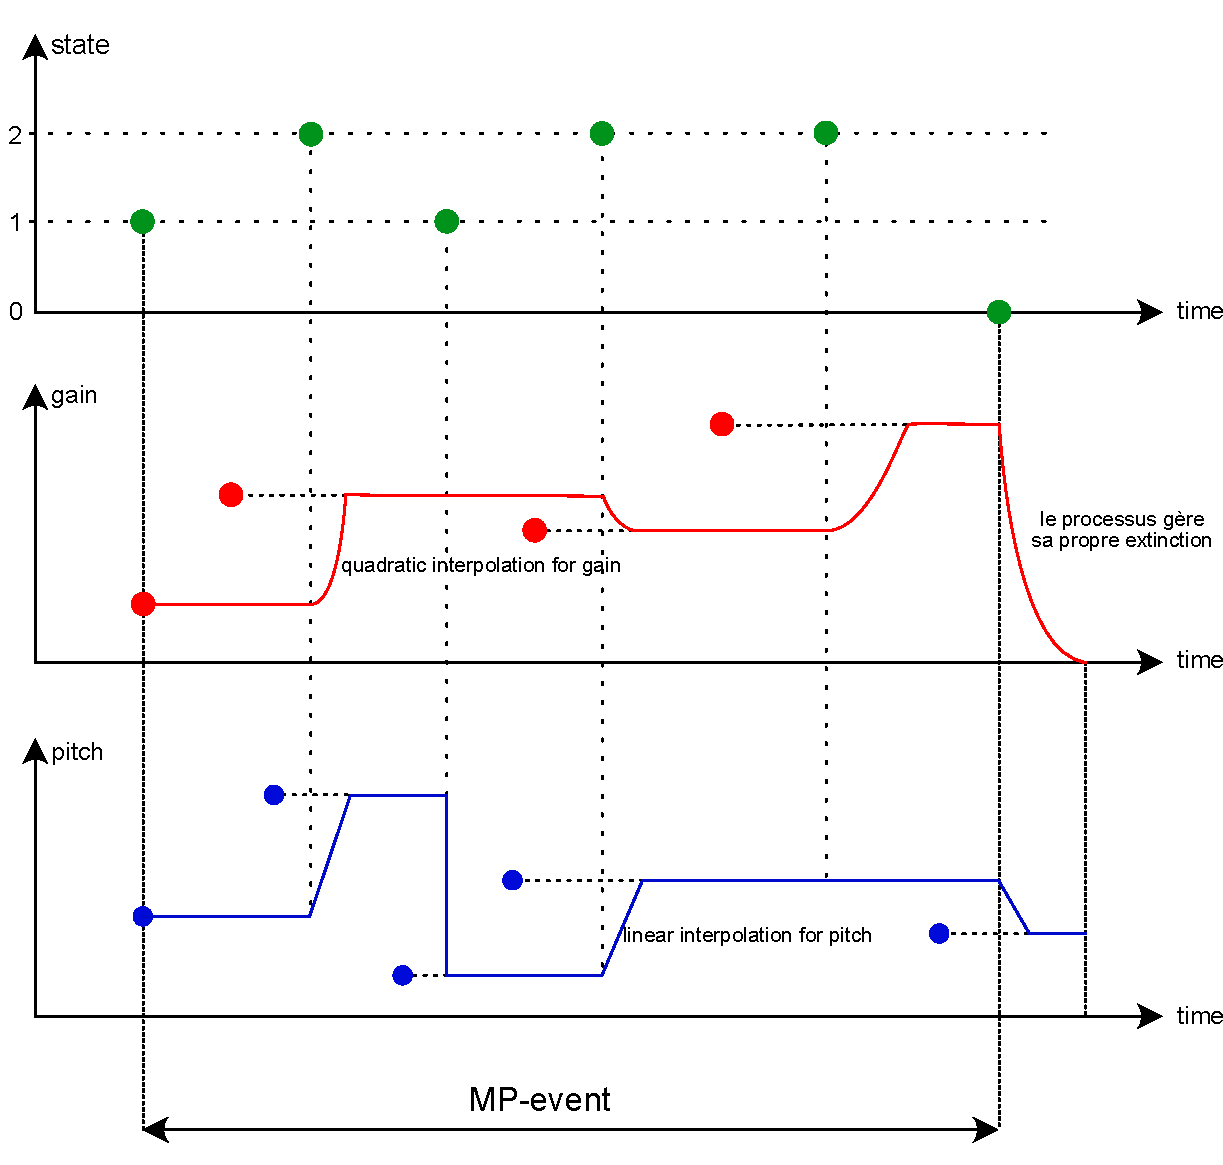
\includegraphics[width=\textwidth]{gfx/04_algorithms/MP-event-model.pdf}
	\caption[Représentation schématique d'un \textit{MP-event}]{Représentation schématique d'un \textit{MP-event}. Les cercles représentent des \textit{MP-messages}, les courbes représentent l'évolution du paramètre dans le processus. Noter que les paramètres ne sont pris en compte que lorsqu'un message \textit{state} est reçu.}
	\label{fig:algorithms:MP-event-model}
\end{figure}
%------------------ Figure : MP-event ---------------------


\subsubsection{Identifiant}

\noindent L'identifiant unique (ID) sert à identifier un \textit{MP-event} tout au long de ses traitements. Le \textit{MP-event} peut provenir d'un capteur physique (e.g. une touche de clavier) ou d'une source virtuelle (e.g. représentant un contact sur une \gls{TUI} ou un produit par un algorithme génératif).
L'ID est présent dans tous les mp-messages pour éviter toute erreur de routage dans le cas où un mp-block reçoit parallèlement des \textit{mp-events} de plusieurs sources indépendantes. Les ID peuvent être définis explicitement --~auquel cas la gestion de conflit d'adressage est laissé à la charge du développeur~-- ou générés de manière unique par un objet dédié : \verb|mp.uID.maker|.

\subsubsection{Etat}

\noindent Le message d'état ``\verb|state|'' est un message réservé qui remplit deux missions :
\vspace{-1em}
\begin{itemize}[noitemsep]
	\item il sert d'horloge asynchrone en déclenchant l'envoi de paramètres au processus;
	\item il spécifie la manière dont le processus doit interpréter ces paramètres.
\end{itemize}

\noindent Les paramètres peuvent ainsi être interprétés de trois façons :

\vspace{-1em}
\begin{itemize}[noitemsep]
	\item \textbf{state 1} : début de modulation de paramètre;
	\item \textbf{state 2} : mise à jour de paramètre;
	\item \textbf{state 0} : fin de modulation de paramètre.	
\end{itemize}

\noindent Le modèle musical sous-jacent envisage un \textit{mp-event} comme la modulation d'un ensemble de paramètres et prend en compte les phénomènes transitoires qui peuvent apparaître au début et/ou à la fin d'une modulation\footnote{ Un exemple évident est l'attaque d'un son, mais en ce qui concerne un processus non-sonore comme le filtrage de données, cela peut concerner l'initialisation du filtre.}. Ces discontinuités peuvent causer des réponses non-linéaires, trop rapides pour être contrôlées manuellement et parfois mieux traitées séparément.\\
\indent Au niveau du processus, ces états peuvent correspondre à l'initialisation de variables internes, l'activation d'un lissage (\textit{portamento}) entre deux valeurs consécutives, le déclenchement d'un processus transitoire spécifique (e.g. l'attaque d'un son), etc. Tout paramètre peut donc être envoyé à un mp-block en spécifiant s'il doit être considéré comme le début, la continuation ou la fin d'une phrase de modulation\footnote{ La confusion entre le \textit{pitch} et l'identifiant de note dans le protocole \gls{MIDI} rend le résultat de la même opération incertain : alors que certains synthétiseurs re-déclencheront la même voix, d'autres alloueront une nouvelle voix et attendront le même nombre de \textit{note-off} qu'il y a eu de \textit{note-on}.}.\\
\indent Ce modèle à trois états semble correspondre par ailleurs aux intentions de la \gls{MMA} qui a annoncé un message de \textit{note-update} dans le futur protocole MIDI-HD\footnote{Rapporté par (dernier accès janvier 2017) : \url{http://www.synthtopia.com/content/2013/01/20/midi-manufacturers-testing-new-high-definition-midi-protocol/}}.\\
\indent Notons toutefois que dans notre cas, le message d'état peut être rattaché à n'importe quel paramètre, ce qui a des conséquences différentes du \gls{MIDI} en ce qui concerne l'allocation de voix. Alors que le premier message \textit{state 1} reçu pour un ID causera l'allocation d'une voix dans le mp-block, le message \textit{state 0} ne libérera pas nécessairement cette voix, cette décision revenant au processus en cours, comme nous le verrons plus loin.

\subsubsection{Guest-list}

\noindent La spécification MP ne suit pas d'organisation hiérarchique telle que les canaux \gls{MIDI} ou les familles d'instruments de \gls{ZIPI}. A la place, elle laisse la possibilité à tout \textit{MP-event} de déclarer une \textit{liste d'invités} (\textit{guestlist}) à la volée. Ces invités pourront avoir accès à la voix allouée à un \textit{MP-event} et contrôler ses paramètres. Cette fonctionnalité nous offre une solution flexible pour le groupement d'événements, permettant un nombre arbitraire de niveaux hiérarchiques, sans pour autant être limité par une relation de subsumption.\\
\indent Cette fonctionnalité peut être utilisée dans le cas de \textit{mp-blocks} génératifs, où l'ID du \textit{MP-event} peut être ajouté à la guestlist des \textit{mp-events} ``enfants''. Ceci permet une modulation cohérente de plusieurs voix associées à des \textit{mp-events} générés par une même source. Des exemples concrets de cette situation sont les pistes \gls{MIDI} ou la hiérarchie orchestre/famille/instrument/note proposée par \gls{ZIPI}. Ils correspondent à un mapping divergent dans le schéma proposé par Rovan, Wanderley, Dubnov et al. \cite{rovan_instrumental_1997}.\\
\indent Un mapping "convergent" est également possible : plusieurs \textit{mp-events} peuvent être déclarés comme guests d'un \textit{MP-event} tiers. Par exemple, un objet graphique virtuel (représenté par un \textit{MP-event}) peut être ``touché'' par plusieurs \textit{mp-events} représentant des contacts sur une surface \gls{TUI}.

\subsubsection{Master-ID}

\noindent Le paramètre guests ne nous laisse toutefois pas un accès aisé à l'ensemble des voix de polyphonies d'un mp-block. A cette fin, un identifiant spécifique indexé à 0, permet ce contrôle global. Il revient implicitement à considérer que le \textit{MP-event} \#0 (nommé master-ID) fait systématiquement partie de la guestlist de tout \textit{MP-event}. Dans le cas où les \textit{mp-events}, ses guests et le master-ID tentent de modifier les mêmes paramètres, le \textit{MP-event} hôte conservera la priorité sur les guests et le master-ID\footnote{On retrouve également cette idée, quoique limitée par les contraintes du \gls{MIDI}, dans la notion de \textit{master channel} du protocole \gls{MPE}}.

\subsubsection{Ordonnancement des mp-messages}

\noindent Le cycle de vie de la voix d'un \textit{MP-event} suit la séquence suivante de \textit{MP-messages} :
\vspace{-1em}
\begin{enumerate}[noitemsep]
	\item envoi des paramètres de début de modulation;
	\item envoi du message state 1;
	\item envoi des paramètres de modulation;
	\item envoi du message state 2;
	\item envoi des paramètres de fin de modulation;
	\item envoi du message state 0.
\end{enumerate}
\noindent Cependant, comme la libération d'une voix ne suit pas nécessairement un message state 0 (dans le cas où le processus a sa propre stratégie d'extinction), il est possible d'envoyer différents messages d'état plusieurs fois durant la durée de vie d'une voix, jusqu'à ce que la voix soit effectivement libérée.

%-----------------------------------------------------------------------------------
\subsection{mp-blocks}

\noindent Un \textit{mp-block} se compose de deux parties (cf. schéma \ref{fig:algorithms:MP-block-model} et implémentation dans Max figure \ref{fig:algorithms:MP-simpleSynth}) : le routeur et le traitement polyphonique que nous décrivons ici.

%------------------ Figure : MP-block ---------------------
\begin{figure}[!htbp]
	\captionsetup{format=plain}
	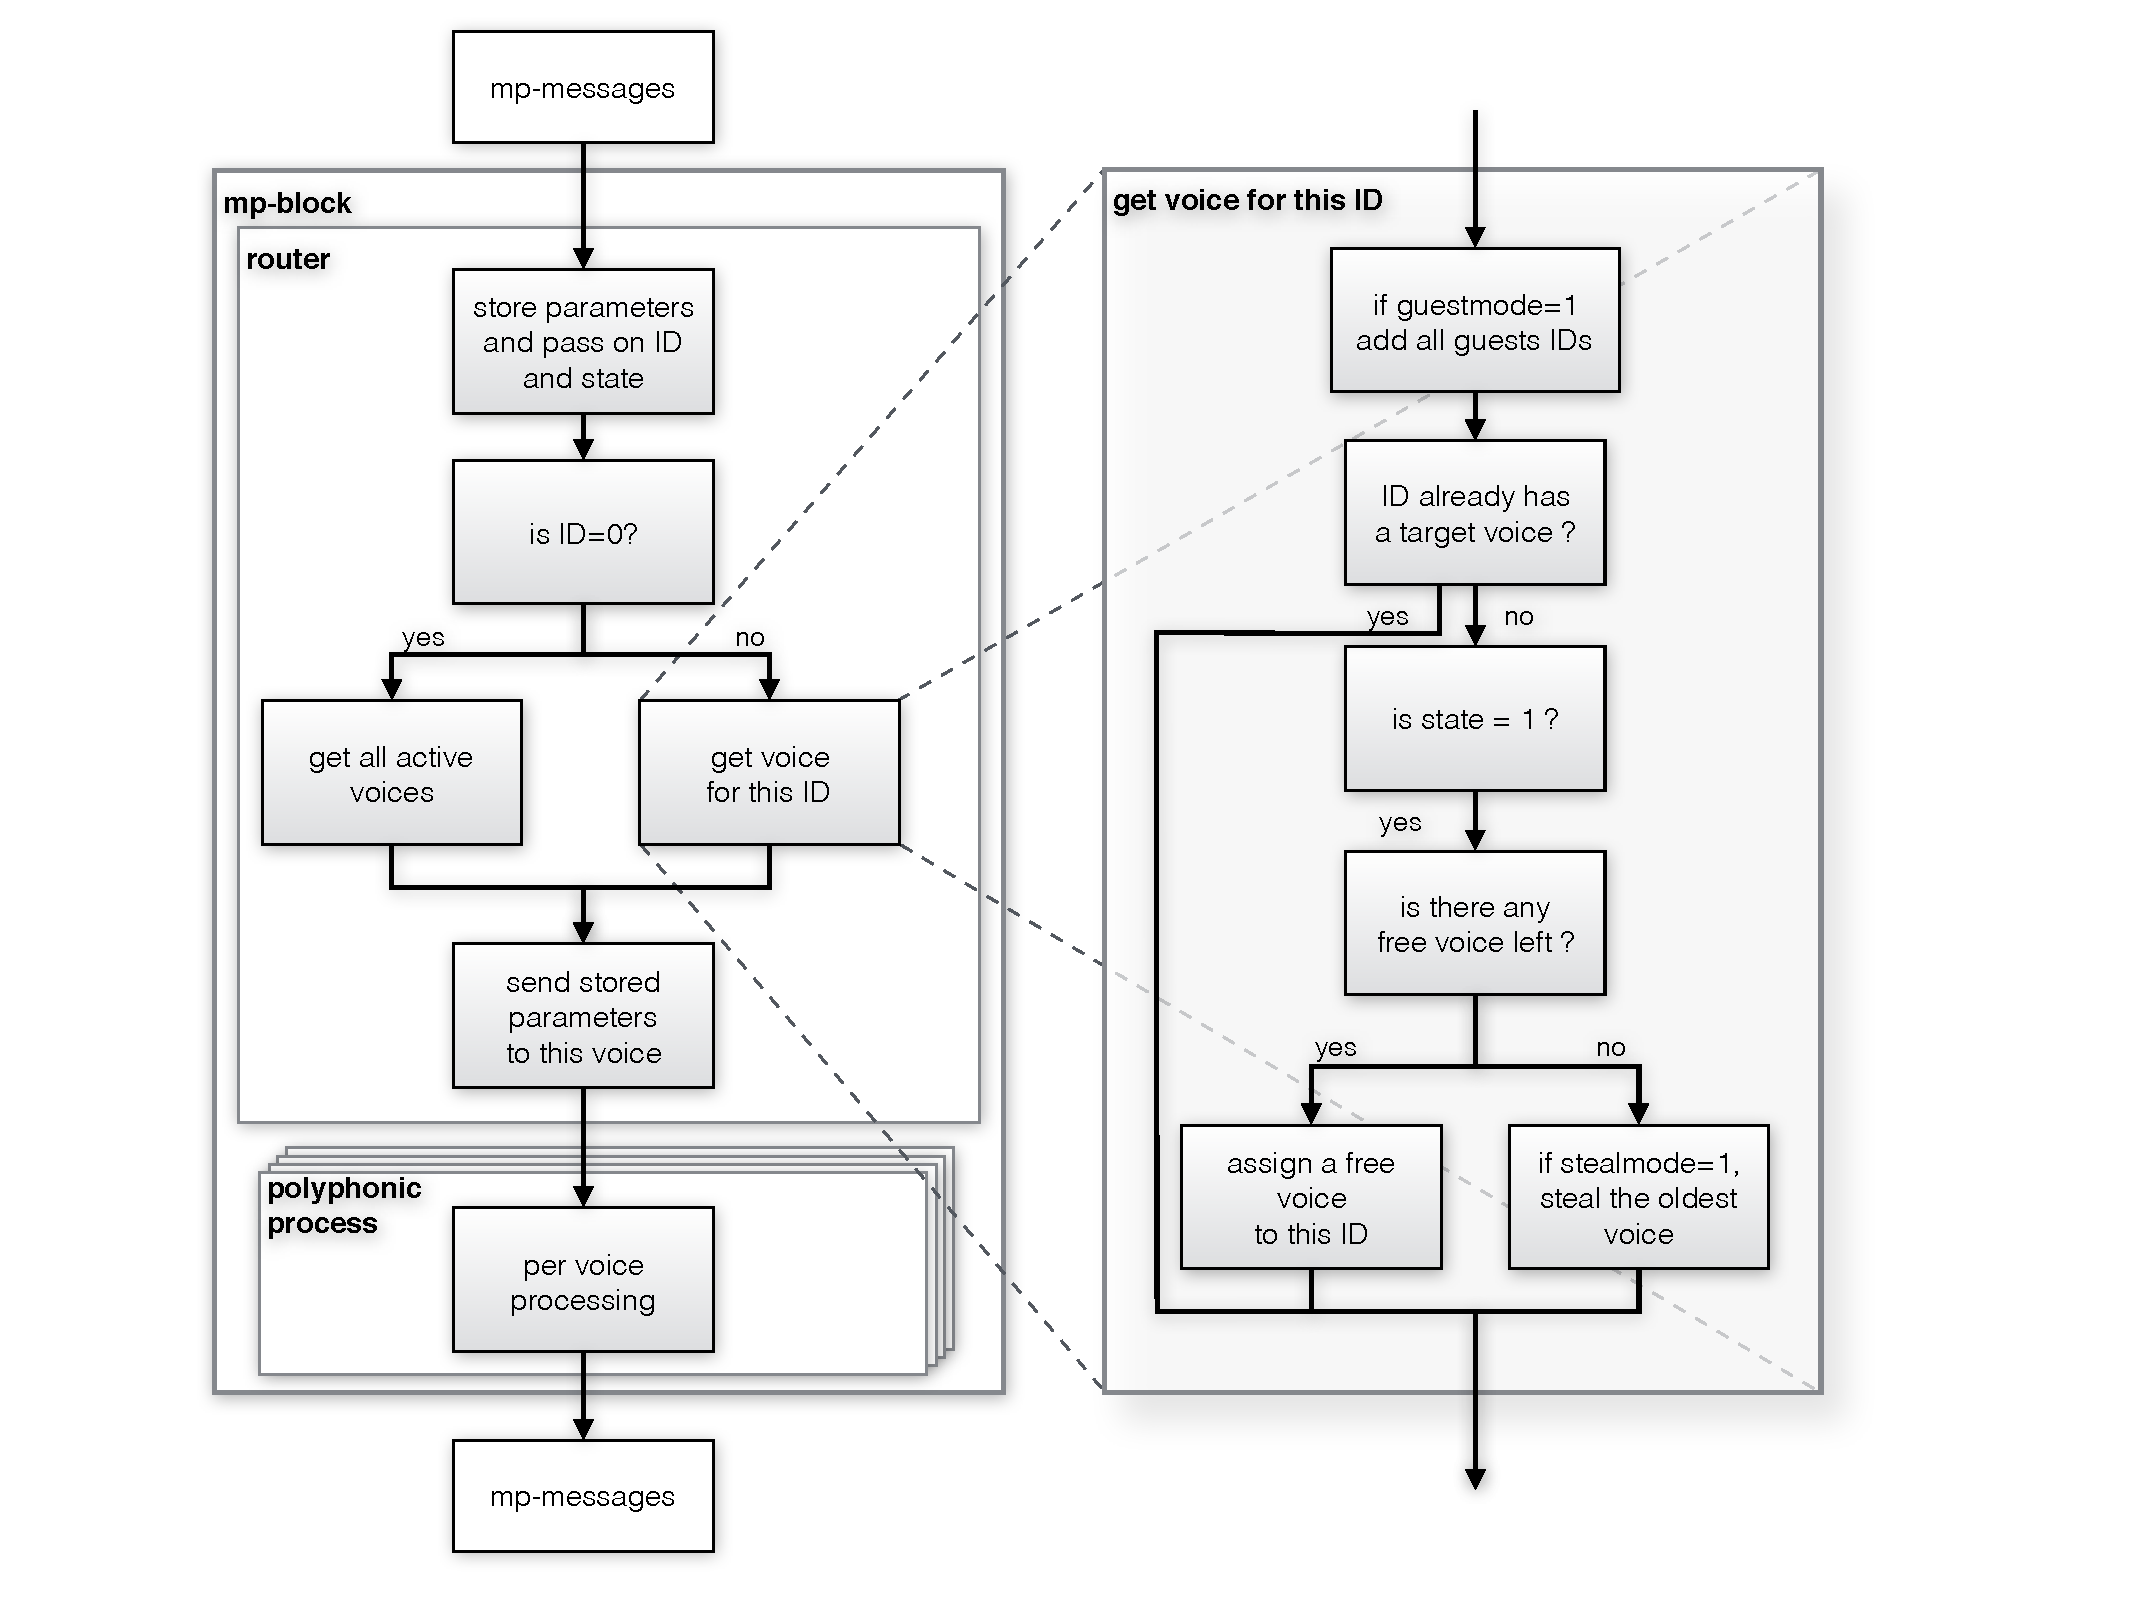
\includegraphics[width=\textwidth]{gfx/04_algorithms/MP-block-model.pdf}
	\caption[Représentation schématique d'un \textit{MP-block}]{Représentation schématique d'un \textit{MP-block} avec le fonctionnement du routeur.}
	\label{fig:algorithms:MP-block-model}
\end{figure}
%------------------ Figure : MP-block ---------------------


\subsubsection{Le routeur}

\noindent Le routeur accomplit les fonctions suivantes :
\vspace{-1em}
\begin{itemize}[noitemsep]
	\item le stockage des paramètres reçu pour un \textit{MP-event};
	\item l'allocation de voix pour un nouvel \textit{MP-event};
	\item l'envoi des paramètres à cette voix;
	\item l'envoi éventuel des paramètres des \textit{guests};
	\item d'enregistrer la libération de la voix;
\end{itemize}

\noindent L'ordonnancement des messages envoyés à la voix de traitement assure une synchronisation du calcul afin qu'il ne soit fait qu'une seule fois. Ainsi, la séquence suivante est envoyée par le routeur à la voix cible :
\vspace{-1em}
\begin{enumerate}[noitemsep]
	\item start X state Y : ce message permet à la voix de se préparer à traiter les paramètres à venir selon l'état Y;
	\item tous les paramètres du master-ID;
	\item tous les paramètres des guests;
	\item tous les paramètres du \textit{MP-event} déclencheur;
	\item end X state Y : ce dernier message clôt la séquence et sert de signal d'horloge déclenchant le calcul.
\end{enumerate}

\noindent L'allocation de voix est réalisée à l'arrivée du premier message \verb|state 1| pour un \textit{MP-event} donné. La libération de la voix intervient quand le processus de traitement indique au routeur qu'il a terminé sa tâche. Trois scénarios sont alors possibles :
\vspace{-1em}
\begin{itemize}[noitemsep]
	\item Le processus se termine dès qu'un message state 0 est reçu. Ce sera le cas, par exemple, pour un processus tel qu'une addition ou un filtre médian. Ce scénario est pris en compte de manière automatique en spécifiant un attribut \verb|@automute 1| au routeur;
	\item Le processus déclenche son extinction à la réception d'un message state 0, typiquement le release d'une enveloppe \gls{ADSR};
	\item Le processus a sa propre durée et peut avoir terminé sa tâche avant ou après avoir reçu un message state 0. C'est le cas, par exemple, lors de la génération d'un signal audio de durée fixe comme un échantillon de percussion.
\end{itemize}

\subsubsection{Traitement par voix}

\noindent Le traitement par voix est effectué par un patch chargé dans les multiples voix d'un objet Max poly\textasciitilde{ }. En dehors des fonctions permettant le traitement à proprement parler, un objet nommé \textit{mp-muter} permet de dispatcher les messages envoyés par le routeur en fonction du message d'état et de renvoyer au routeur l'information de fin de tâche que le processus doit fournir dans le cas où il possède une extinction propre (mode \verb|@automute 0|). Ce principe est exposé sur la figure \ref{fig:algorithms:MP-simpleSynth-inside}, dans laquelle l'objet Max \verb|adsr~| vient notifier l'objet \textit{mp.muter} de la fin de l'enveloppe.

%------------------ Figure : simple synth ---------------------
\begin{figure}[!htbp]
	\captionsetup{format=plain}%
	\centering
	\begin{minipage}[t]{0.5035\textwidth}
		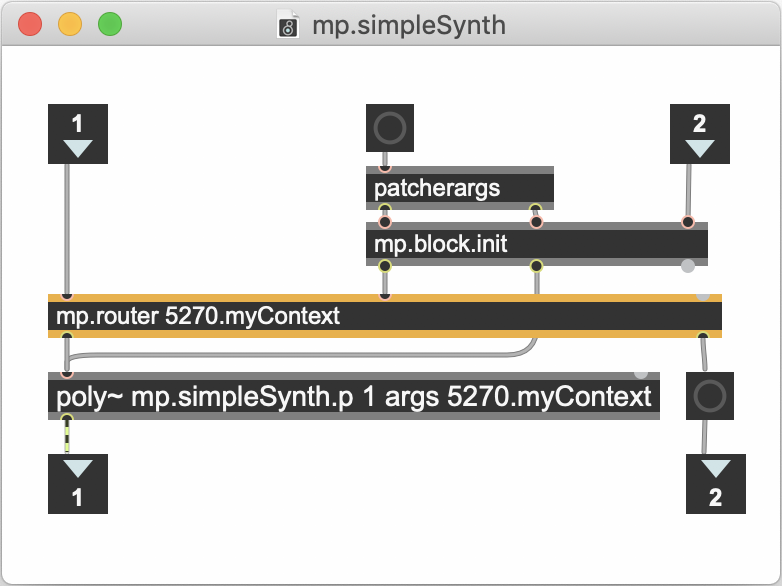
\includegraphics[width=\linewidth]{gfx/04_algorithms/MP-reallySimpleSynth.png}
		\caption[mp.simpleSynth : encapsulation de la synthèse]{mp.simpleSynth : routeur et encapsulation de la synthèse.}
		\label{fig:algorithms:MP-simpleSynth}
	\end{minipage}
	\hspace{.01\linewidth}
	\begin{minipage}[t]{0.4635\textwidth}
	  	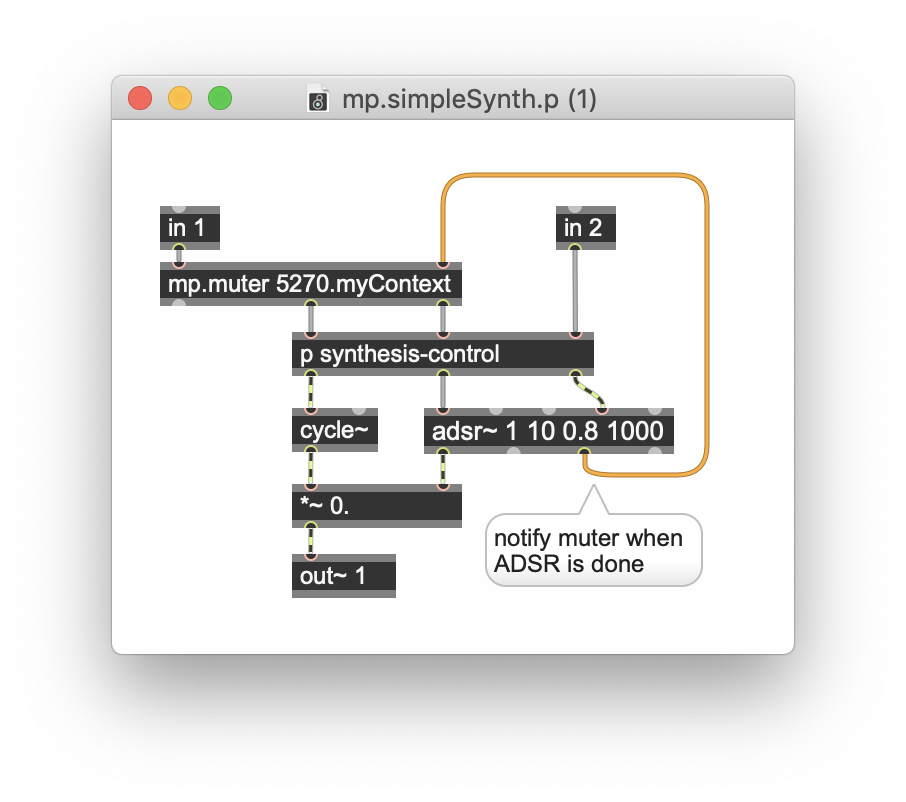
\includegraphics[width=\linewidth]{gfx/04_algorithms/MP-reallySimpleSynth-inside.png}
		\caption[mp.simpleSynth : patcher de synthèse]{mp.simpleSynth : patcher de synthèse. Le route est notifié de la fin d'activité de l'envoi d'un message ``mute'' par l'objet ADSR.}
		\label{fig:algorithms:MP-simpleSynth-inside}
	\end{minipage}
\end{figure}
%------------------ Figure : simple synth ---------------------


\subsubsection{Paramètres d'un mp-block}

\noindent Les \textit{mp-blocks} répondent à une liste de paramètres contrôlant le processus de traitement par voix. Ces paramètres sont stockés par identifiant dans le routeur jusqu'à ce qu'un message d'état soit reçu. Ce message entrainera l'allocation d'une voix (si disponible et si elle n'est pas déjà active), puis l'envoi de tous les paramètres partageant cet identifiant à cette voix.\\
\indent Il est possible d'envoyer d'autres paramètres que ceux contrôlant le processus. Dans ce cas il traverseront le \textit{mp-block} inchangés, tout en restant synchrones avec d'éventuels autres paramètres générés par le processus qu'ils traversent. Dans le cas où ce processus génère de nouveaux \textit{mp-events}, ces paramètres peuvent automatiquement être ajoutés à chaque \textit{MP-event} généré, en une sorte d'héritage similaire à celui opéré par la librairie ``o.'' décrit dans \cite{goudard_dynamic_2011} (TODO :renvoyer plutôt à la section qui parle des MID).


%-----------------------------------------------------------------------------------
\subsection{Exemples}

\noindent Les exemples proposés dans cette section donnent des cas concrets d'utilisation du système MP. Ils sont implémentés dans le logiciel Max.

\subsubsection{Mapping encapsulé}
\noindent Cet exemple (figure TODO ref) montre l'utilisation la plus simple du système MP. À partir de données \gls{TUIO} issues d'une interface \textit{multitouch}, on contrôle les valeurs de vélocité et de cutoff sur l'axe vertical tandis que l'axe horizontal contrôle le pitch.
Le module mp-embedded-mapping-demoSynth est constitué d'un routeur et d'un objet poly contenant à la fois le mapping et la synthèse. Ici, l'avantage d'utiliser MP est de bénéficier d'un système d'adressage similaire au \gls{MPE} sans être limité par le typage, la précision et l'espace de nommage des données.

\subsubsection{Mapping dé-encapsulé}

\noindent Dans cet exemple (figure TODO ref), nous avons sorti tout le mapping en dehors du module de synthèse. Examinons quelques éléments de ce patch :
\vspace{-1em}
\begin{itemize}[noitemsep]
	\item à gauche, le module \textit{mp.note2chord} génère un ensemble de \textit{mp-events} "enfants". Le premier niveau en génère deux et le deuxième niveau en génère 3. Le résultat final est la génération d'un accord de six notes à partir d'un seul \textit{MP-event};
	\item à droite, le \textit{MP-event} venant de \textit{mp.TUIO.input} est envoyé sur deux chemins où ses valeurs sont mises à l'échelle par le module mp-scale pour définir la fréquence et l'offset d'un LFO respectivement. Le \gls{LFO} contrôlera ensuite la fréquence de coupure d'un filtre passe-bas du module de synthèse;
	\item nous avons deux occurrences d'un contrôle global avec le Master-ID : une pour le paramètre \textit{depth} du LFO et une pour la transposition du deuxième étage \textit{note2chord};
	\item en dernier lieu, nous dirigeons les messages résultants de ces deux chemins vers un système de représentation graphique. La position d'objets graphiques est assignée aux valeurs de pitch des \textit{mp-events} générés, tandis que leur couleur est associée au \textit{MP-event} parent. Ceci résulte en une représentation graphique de toutes les hauteurs en tant qu'objets dont la couleur nous dit à quelle source commune (ici le contact d'un doigt sur un écran) ils sont rattachés
\end{itemize}

\subsubsection*{Mapping many[guests]-to-one}
\noindent Alors que les exemples précédents nous montrent une utilisation de la guestlist comme hiérarchie de subsumption, ce dernier exemple fournit un exemple concret de relation \textit{many-to-one}. Ici, les \textit{mp-events} arrivant d'une \gls{TUI} et représentant la position des doigts (les points) causeront l'apparition d'un arc si la distance entre eux passe sous un certain seuil.\\
\indent Le \textit{MP-event} « arc » ainsi généré aura les deux \textit{mp-events} « points » dans sa guestlist, de telle sorte que toute modification sur les points affectera le traitement aval du \textit{MP-event} représenté par l'arc.

\subsection{Limitations et optimisations}

\noindent Séparer les différents processus de traitement d'un design d'interaction polyphonique a l'avantage de permettre une meilleure modularité et, par suite, une meilleure stabilité des processus mis en œuvre qui n'auront pas à être modifiés en interne. Le choix a également été fait de ne pas s'appuyer sur une mémoire globale (e.g. pour sauver la guestlist) de sorte que les \textit{mp-blocks} soient réellement indépendants et autonomes et que le design d'interaction général puisse être réparti sur plusieurs applications et/ou machines en réseau.\\
\indent Cependant, cette modularité a un coût et est probablement moins efficace que d'inclure tous les traitements nécessaires dans les traitements ad-hoc. Certaines optimisations peuvent être réalisées pour des processus ne nécessitant pas de mémoire interne (e.g. une mise à l'échelle statique), pour lesquels il n'est pas nécessaire d'allouer des voix. Cela se fait cependant au prix de certaines fonctionnalités (pas d'utilisation du \textit{master-ID} possible dans ce cas).\\
\indent De plus, le framework MP a entièrement été réalisé à l'aide d'objets natifs Max et pourrait sûrement être optimisé en le portant sous la forme d'objets compilés.

\subsection{Conclusions}
\noindent Le système MP permet la connexion modulaire de processus polyphoniques. Bien qu'il soit encore à un stade précoce, ce système permet d'explorer de nouveaux modèles de lutherie numérique, impliquant notamment des contrôleurs expressifs et des interfaces multi-touch ou composites.
Ces développements sont également menés pour répondre à d'autres questions telles que la représentation et l'ergonomie des processus polyphoniques que présentés dans la section suivante et les chapitres suivants.

%%%%%%%%%%%%%%%%%%%%%%%%%%%%%%%%%%%%%%%%%
\section{Sagrada : extension de MP au DSP}
\label{sec:algorithms:sagrada}

%----------------------------------------------------------------------------------------------------------
\subsection{Motivations et contexte}
Possibilité de délencher des grains à une fréquence égale au sample rate (par rapport à SR/2 dans le cas d'un déclenchement au zéro-crossing tel que pratiqué dans GMU)
%----------------------------------------------------------------------------------------------------------
\subsection{Implémentation}
\subsubsection{Horloge et assignation de voix}
Sagrada fonctionne selon le principe que chaque impulsion arrivant sur une entrée audio incrémente un compteur qui définit la voix de polyphonie qui sera activée. Un objet Max dédié ``sagrada.trigger\textasciitilde{ }'' peut ainsi être controlé soit de manière asynchrone (e.g. en transformant un message \gls{MIDI} en impulsion (delta de Kronecker), soit en envoyant un train d'impulsion synchrone contrôlé en fréquence.

Notons qu'il est ainsi possible de déclencher plusieurs grain

\subsubsection{Busy}
Les synthètiseurs polyphoniques peuvent généralement fonctionner sous deux modes: soit ils permettent qu'une nouvelle voix soit attribuée en volant éventuellement une .
L'utilisation d'un fonctionnement par ``buffer'' comme dans le cas de la librairie GMU permet de savoir à l'avance le temps que va durer un grain

%----------------------------------------------------------------------------------------------------------
\subsection{Performances comparée}
bufgranul : permet de générer des grains à une fréquence double. Approche modulaire permetttant l'application de n'importe quel effet par grain.

gen\textasciitilde{ } OLA

granularized

ftm

mc.*


\section*{extra material}

la production de hauteur dans les instruments acoustique est systématiquement liée à un phénomène de résonance, c'est à dire un phénomène de bouclage, de feedback. 

La sélection de différentes hauteurs peut ensuite être obtenue 
- en jouant sur une multitude d'éléments accordés différemment (les cordes d'une harpe, les lames
d'un marimba, etc.) ;
- en modifiant les caractéristiques d'un élément résonnant, le plus souvent sa longueur (tube des
instruments à vent, corde d'un violoncelle) ;
- en sélectionnant des harmoniques précis d'un son riche (didgeridoo, chant diphonique).


Dans les DIMs la production de hauteur est essentiellement possible de deux manières: 
- par la lecture, éventuellement en boucle, d'une table d'onde
- par le délai de réinjection d'un filtre résonnant (synthèse soustractive, Karplus, etc.)
- par un calcul mathématique impliquant des fonctions périodiques (telles que les sinus dans la FFT)

L'acoustique physique présente naturellement des non-linéarité qui contribuent à la richesse du son et l'identité de son timbre. L'électronique analogique permet également d'obtenir —sur l'espace restreint d'un signal mono-dimensionnel par rapport à l'acoustique physique généralement bi- ou tri-dimensionnelle— des systèmes résonants non-linéaire et stables, via l'utilisation de composants électronique passifs.

Les choses sont plus compliquées pour le son numérique, s'il est possible d'obtenir des systèmes résonant stables (en maintenant les pôles dans le cercle unitaire du le plan complexe), la garantie de stabilité devient très complexe à évaluer dès que l'on introduit de la non-linéarité.
Malgré de récentes avancées dans ce domaine (cf. travaux de Thomas Hélie sur les systèmes Hamiltoniens à ports)


\iquote{Mapping describes the way a control is con- nected to a variable. But as instruments be- come more complex to include large amounts of data, context sensitivity, and music as well as sound-generating capabilities, the concept of mapping becomes more abstract and does not describe the more complex realities of elec- tronic instruments.} Chadabe in \cite{chadabe_limitations_2002}